\documentclass[12pt, a4paper]{article}
\usepackage[left=2.54cm, right=2.54cm, bottom=2.54cm, top=2.54cm]{geometry}
\linespread{1}
\usepackage{setspace}
\usepackage[utf8]{inputenc}
\usepackage{blindtext}
\usepackage[T1]{fontenc}
\usepackage{xcolor}
\usepackage{amsfonts}
\usepackage{amsmath}
\usepackage{amssymb}
\usepackage{fancyhdr}
\usepackage{tikz}
\pagestyle{fancy}
\fancyhead{}
\fancyfoot{}
\fancyfoot[R]{\thepage}
\renewcommand{\headrulewidth}{2pt}
\renewcommand{\footrulewidth}{2pt}
\usepackage{graphicx}
\usepackage{multicol}
\graphicspath{ {./img/} }

\title{Laporan PBO Tugas 2}
\author{5025241134 Gilbran Mahavikia Raja}
\date{\today}

\begin{document}
\maketitle

\section{Russian Year 5 Problem}

\includegraphics[scale=0.3]{soal.png}

Dalam soal diberikan sebuah daftar $T$ berisi $N$ angka $(1 \leq N \leq  10^4)$, setiap $T[i]$ berada dalam rentang 1 hingga 169, dan diketahui bahwa terdapat tepat dua angka dalam daftar yang jika dijumlahkan menghasilkan 100.

\section{Identifikasi Masalah}

Masalahnya adalah mencari dua unsur dalam array yang jumlahnya sama dengan target tertentu $(100)$. Domain klasik ini disebut “two-sum”, dengan kondisi:

\begin{itemize}
  \item $N \leq 10^4$, sehingga solusi $O(N^2)$ masih mungkin tetapi mungkin terancam waktu tergantung konstanta, sedangkan $O(N)$ sangat ideal.
  \item Nilai-nilai kecil (maks $169$), memperbolehkan juga pendekatan counting atau lookup tabel kecil.
  \item Dinyatakan solusi unik, jadi hanya satu pasangan yang tepat.
  \item Dalam Komentar di soal ada yang mengeluhkan solusi $O(N^2)$ menghasilkan WA sementara versi berbasis hashmap AC. 
\end{itemize}



\section{Solusi dan implementasi pada C++}
Solusi masalah MGSINFOB bisa diselesaikan dengan memanfaatkan $unordered\_map$ di C++ untuk melakukan pencarian pasangan bilangan secara cepat. Caranya, kita buat sebuah $unordered\_map<int, int>$ yang berfungsi menyimpan nilai dari elemen array sebagai key dan indeksnya ($1-$based) sebagai value. Kemudian, saat kita melakukan iterasi pada array, untuk setiap elemen $x = T[i]$ kita hitung nilai pasangan yang dibutuhkan, yaitu $y = 100 - x$. Jika $y$ sudah ada di dalam $unordered\_map$, berarti kita telah menemukan pasangan angka yang jumlahnya $100$, maka langsung cetak indeks $y$ (yang sudah tersimpan di map) dan indeks $x$ saat ini $(i+1)$. Karena $unordered\_map$ mendukung operasi pencarian (find) dalam waktu konstan rata-rata $O(1)$, seluruh algoritma berjalan dalam kompleksitas $O(N)$. Setelah mencetak kedua indeks tersebut, program bisa langsung berhenti karena soal menjamin solusi unik. Dengan pendekatan ini, kita tidak perlu lagi menggunakan nested loop seperti pada brute-force, sehingga lebih efisien dan aman dari kesalahan urutan indeks.\\ \\
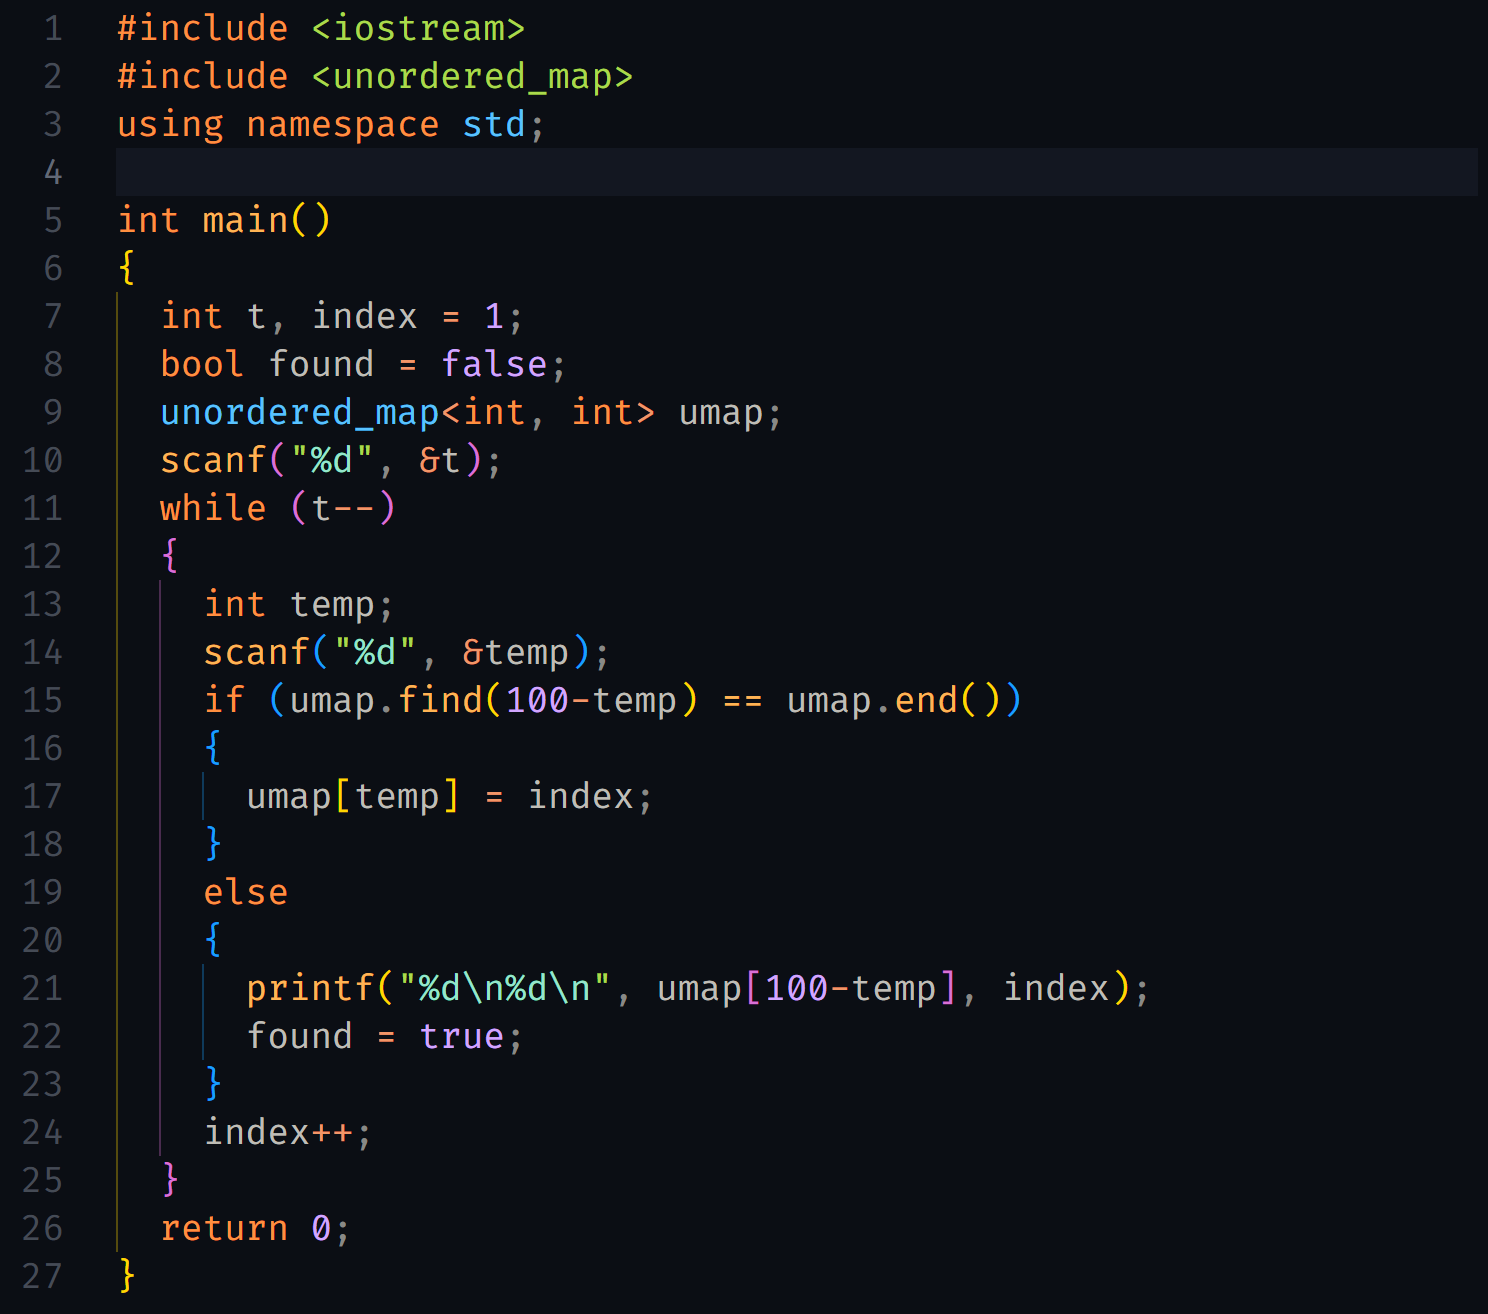
\includegraphics[scale=0.3]{kode.png}

\section{Bukti}
Berikut adalah bukti bahwa solusi saya mendapatkan verdict \textbf{Accepted}.\\

\includegraphics[scale=0.19]{buktiAC.png}
\end{document}